%% This demo file is intended to serve as a ``starter file'' for 
%% IEEE Journal of Electromagnetics, RF and Microwaves in Medicine and
%% Biology (JERM) papers produced under \LaTeX\ using modified IEEEtran.cls
%% file in order to meet the special typesetting requirements of JERM.

%% Modified by Zhengyu Peng based on bare_jrnl.tex from Michael Shell 
%% Support sites:
%% https://github.com/rookiepeng/JERM-LaTeX-Template
%% http://www.michaelshell.org/tex/ieeetran/
%% http://www.ctan.org/pkg/ieeetran
%% and
%% http://www.ieee.org/

%%*************************************************************************
%% Legal Notice:
%% This code is offered as-is without any warranty either expressed or
%% implied; without even the implied warranty of MERCHANTABILITY or
%% FITNESS FOR A PARTICULAR PURPOSE! 
%% User assumes all risk.
%% In no event shall the IEEE or any contributor to this code be liable for
%% any damages or losses, including, but not limited to, incidental,
%% consequential, or any other damages, resulting from the use or misuse
%% of any information contained here.
%%
%% All comments are the opinions of their respective authors and are not
%% necessarily endorsed by the IEEE.
%%
%% This work is distributed under the LaTeX Project Public License (LPPL)
%% ( http://www.latex-project.org/ ) version 1.3, and may be freely used,
%% distributed and modified. A copy of the LPPL, version 1.3, is included
%% in the base LaTeX documentation of all distributions of LaTeX released
%% 2003/12/01 or later.
%% Retain all contribution notices and credits.
%% ** Modified files should be clearly indicated as such, including  **
%% ** renaming them and changing author support contact information. **
%%*************************************************************************

% *** Authors should verify (and, if needed, correct) their LaTeX system  ***
% *** with the testflow diagnostic prior to trusting their LaTeX platform ***
% *** with production work. The IEEE's font choices and paper sizes can   ***
% *** trigger bugs that do not appear when using other class files.       ***                          ***

\documentclass[journal,twocolumn,letterpaper]{IEEEJERM}
%
% If IEEEtran.cls has not been installed into the LaTeX system files,
% manually specify the path to it like:
% \documentclass[journal]{../sty/IEEEtran}

% Some very useful LaTeX packages include:
% (uncomment the ones you want to load)

% *** MISC UTILITY PACKAGES ***
%
%\usepackage{ifpdf}
% Heiko Oberdiek's ifpdf.sty is very useful if you need conditional
% compilation based on whether the output is pdf or dvi.
% usage:
% \ifpdf
%   % pdf code
% \else
%   % dvi code
% \fi
% The latest version of ifpdf.sty can be obtained from:
% http://www.ctan.org/pkg/ifpdf
% Also, note that IEEEtran.cls V1.7 and later provides a builtin
% \ifCLASSINFOpdf conditional that works the same way.
% When switching from latex to pdflatex and vice-versa, the compiler may
% have to be run twice to clear warning/error messages.


% *** CITATION PACKAGES ***
%
%\usepackage{cite}
% cite.sty was written by Donald Arseneau
% V1.6 and later of IEEEtran pre-defines the format of the cite.sty package
% \cite{} output to follow that of the IEEE. Loading the cite package will
% result in citation numbers being automatically sorted and properly
% "compressed/ranged". e.g., [1], [9], [2], [7], [5], [6] without using
% cite.sty will become [1], [2], [5]--[7], [9] using cite.sty. cite.sty's
% \cite will automatically add leading space, if needed. Use cite.sty's
% noadjust option (cite.sty V3.8 and later) if you want to turn this off
% such as if a citation ever needs to be enclosed in parenthesis.
% cite.sty is already installed on most LaTeX systems. Be sure and use
% version 5.0 (2009-03-20) and later if using hyperref.sty.
% The latest version can be obtained at:
% http://www.ctan.org/pkg/cite
% The documentation is contained in the cite.sty file itself.


% *** GRAPHICS RELATED PACKAGES ***
%
\ifCLASSINFOpdf
  % \usepackage[pdftex]{graphicx}
  % declare the path(s) where your graphic files are
  % \graphicspath{{../pdf/}{../jpeg/}}
  % and their extensions so you won't have to specify these with
  % every instance of \includegraphics
  % \DeclareGraphicsExtensions{.pdf,.jpeg,.png}
\else
  % or other class option (dvipsone, dvipdf, if not using dvips). graphicx
  % will default to the driver specified in the system graphics.cfg if no
  % driver is specified.
  % \usepackage[dvips]{graphicx}
  % declare the path(s) where your graphic files are
  % \graphicspath{{../eps/}}
  % and their extensions so you won't have to specify these with
  % every instance of \includegraphics
  % \DeclareGraphicsExtensions{.eps}
\fi
% graphicx was written by David Carlisle and Sebastian Rahtz. It is
% required if you want graphics, photos, etc. graphicx.sty is already
% installed on most LaTeX systems. The latest version and documentation
% can be obtained at: 
% http://www.ctan.org/pkg/graphicx
% Another good source of documentation is "Using Imported Graphics in
% LaTeX2e" by Keith Reckdahl which can be found at:
% http://www.ctan.org/pkg/epslatex
%
% latex, and pdflatex in dvi mode, support graphics in encapsulated
% postscript (.eps) format. pdflatex in pdf mode supports graphics
% in .pdf, .jpeg, .png and .mps (metapost) formats. Users should ensure
% that all non-photo figures use a vector format (.eps, .pdf, .mps) and
% not a bitmapped formats (.jpeg, .png). The IEEE frowns on bitmapped formats
% which can result in "jaggedy"/blurry rendering of lines and letters as
% well as large increases in file sizes.
%
% You can find documentation about the pdfTeX application at:
% http://www.tug.org/applications/pdftex


% *** MATH PACKAGES ***
%
%\usepackage{amsmath}
% A popular package from the American Mathematical Society that provides
% many useful and powerful commands for dealing with mathematics.
%
% Note that the amsmath package sets \interdisplaylinepenalty to 10000
% thus preventing page breaks from occurring within multiline equations. Use:
%\interdisplaylinepenalty=2500
% after loading amsmath to restore such page breaks as IEEEtran.cls normally
% does. amsmath.sty is already installed on most LaTeX systems. The latest
% version and documentation can be obtained at:
% http://www.ctan.org/pkg/amsmath


% *** SPECIALIZED LIST PACKAGES ***
%
%\usepackage{algorithmic}
% algorithmic.sty was written by Peter Williams and Rogerio Brito.
% This package provides an algorithmic environment fo describing algorithms.
% You can use the algorithmic environment in-text or within a figure
% environment to provide for a floating algorithm. Do NOT use the algorithm
% floating environment provided by algorithm.sty (by the same authors) or
% algorithm2e.sty (by Christophe Fiorio) as the IEEE does not use dedicated
% algorithm float types and packages that provide these will not provide
% correct IEEE style captions. The latest version and documentation of
% algorithmic.sty can be obtained at:
% http://www.ctan.org/pkg/algorithms
% Also of interest may be the (relatively newer and more customizable)
% algorithmicx.sty package by Szasz Janos:
% http://www.ctan.org/pkg/algorithmicx


% *** ALIGNMENT PACKAGES ***
%
%\usepackage{array}
% Frank Mittelbach's and David Carlisle's array.sty patches and improves
% the standard LaTeX2e array and tabular environments to provide better
% appearance and additional user controls. As the default LaTeX2e table
% generation code is lacking to the point of almost being broken with
% respect to the quality of the end results, all users are strongly
% advised to use an enhanced (at the very least that provided by array.sty)
% set of table tools. array.sty is already installed on most systems. The
% latest version and documentation can be obtained at:
% http://www.ctan.org/pkg/array


% IEEEtran contains the IEEEeqnarray family of commands that can be used to
% generate multiline equations as well as matrices, tables, etc., of high
% quality.


% *** SUBE PACKAGES ***
%\ifCLASSOPTIONcompsoc
%  \usepackage[caption=false,font=normalsize,labelfont=sf,textfont=sf]{subfig}
%\else
%  \usepackage[caption=false,font=footnotesize]{subfig}
%\fi
% subfig.sty, written by Steven Douglas Cochran, is the modern replacement
% for subfigure.sty, the latter of which is no longer maintained and is
% incompatible with some LaTeX packages including fixltx2e. However,
% subfig.sty requires and automatically loads Axel Sommerfeldt's caption.sty
% which will override IEEEtran.cls' handling of captions and this will result
% in non-IEEE style figure/table captions. To prevent this problem, be sure
% and invoke subfig.sty's "caption=false" package option (available since
% subfig.sty version 1.3, 2005/06/28) as this is will preserve IEEEtran.cls
% handling of captions.
% Note that the Computer Society format requires a larger sans serif font
% than the serif footnote size font used in traditional IEEE formatting
% and thus the need to invoke different subfig.sty package options depending
% on whether compsoc mode has been enabled.
%
% The latest version and documentation of subfig.sty can be obtained at:
% http://www.ctan.org/pkg/subfig


% *** FLOAT PACKAGES ***
%
%\usepackage{fixltx2e}
% fixltx2e, the successor to the earlier fix2col.sty, was written by
% Frank Mittelbach and David Carlisle. This package corrects a few problems
% in the LaTeX2e kernel, the most notable of which is that in current
% LaTeX2e releases, the ordering of single and double column floats is not
% guaranteed to be preserved. Thus, an unpatched LaTeX2e can allow a
% single column figure to be placed prior to an earlier double column
% figure.
% Be aware that LaTeX2e kernels dated 2015 and later have fixltx2e.sty's
% corrections already built into the system in which case a warning will
% be issued if an attempt is made to load fixltx2e.sty as it is no longer
% needed.
% The latest version and documentation can be found at:
% http://www.ctan.org/pkg/fixltx2e


%\usepackage{stfloats}
% stfloats.sty was written by Sigitas Tolusis. This package gives LaTeX2e
% the ability to do double column floats at the bottom of the page as well
% as the top. (e.g., "\begin{figure*}[!b]" is not normally possible in
% LaTeX2e). It also provides a command:
%\fnbelowfloat
% to enable the placement of footnotes below bottom floats (the standard
% LaTeX2e kernel puts them above bottom floats). This is an invasive package
% which rewrites many portions of the LaTeX2e float routines. It may not work
% with other packages that modify the LaTeX2e float routines. The latest
% version and documentation can be obtained at:
% http://www.ctan.org/pkg/stfloats
% Do not use the stfloats baselinefloat ability as the IEEE does not allow
% \baselineskip to stretch. Authors submitting work to the IEEE should note
% that the IEEE rarely uses double column equations and that authors should try
% to avoid such use. Do not be tempted to use the cuted.sty or midfloat.sty
% packages (also by Sigitas Tolusis) as the IEEE does not format its papers in
% such ways.
% Do not attempt to use stfloats with fixltx2e as they are incompatible.
% Instead, use Morten Hogholm'a dblfloatfix which combines the features
% of both fixltx2e and stfloats:
%
% \usepackage{dblfloatfix}
% The latest version can be found at:
% http://www.ctan.org/pkg/dblfloatfix


%\ifCLASSOPTIONcaptionsoff
%  \usepackage[nomarkers]{endfloat}
% \let\MYoriglatexcaption\caption
% \renewcommand{\caption}[2][\relax]{\MYoriglatexcaption[#2]{#2}}
%\fi
% endfloat.sty was written by James Darrell McCauley, Jeff Goldberg and 
% Axel Sommerfeldt. This package may be useful when used in conjunction with 
% IEEEtran.cls'  captionsoff option. Some IEEE journals/societies require that
% submissions have lists of figures/tables at the end of the paper and that
% figures/tables without any captions are placed on a page by themselves at
% the end of the document. If needed, the draftcls IEEEtran class option or
% \CLASSINPUTbaselinestretch interface can be used to increase the line
% spacing as well. Be sure and use the nomarkers option of endfloat to
% prevent endfloat from "marking" where the figures would have been placed
% in the text. The two hack lines of code above are a slight modification of
% that suggested by in the endfloat docs (section 8.4.1) to ensure that
% the full captions always appear in the list of figures/tables - even if
% the user used the short optional argument of \caption[]{}.
% IEEE papers do not typically make use of \caption[]'s optional argument,
% so this should not be an issue. A similar trick can be used to disable
% captions of packages such as subfig.sty that lack options to turn off
% the subcaptions:
% For subfig.sty:
% \let\MYorigsubfloat\subfloat
% \renewcommand{\subfloat}[2][\relax]{\MYorigsubfloat[]{#2}}
% However, the above trick will not work if both optional arguments of
% the \subfloat command are used. Furthermore, there needs to be a
% description of each subfigure *somewhere* and endfloat does not add
% subfigure captions to its list of figures. Thus, the best approach is to
% avoid the use of subfigure captions (many IEEE journals avoid them anyway)
% and instead reference/explain all the subfigures within the main caption.
% The latest version of endfloat.sty and its documentation can obtained at:
% http://www.ctan.org/pkg/endfloat
%
% The IEEEtran \ifCLASSOPTIONcaptionsoff conditional can also be used
% later in the document, say, to conditionally put the References on a 
% page by themselves.


% *** PDF, URL AND HYPERLINK PACKAGES ***
%
%\usepackage{url}
% url.sty was written by Donald Arseneau. It provides better support for
% handling and breaking URLs. url.sty is already installed on most LaTeX
% systems. The latest version and documentation can be obtained at:
% http://www.ctan.org/pkg/url
% Basically, \url{my_url_here}.


% *** Do not adjust lengths that control margins, column widths, etc. ***
% *** Do not use packages that alter fonts (such as pslatex).         ***
% There should be no need to do such things with IEEEtran.cls V1.6 and later.
% (Unless specifically asked to do so by the journal or conference you plan
% to submit to, of course. )


\usepackage{times,amsmath,epsfig}
\usepackage{fancyhdr}
\usepackage{amsmath}
\usepackage{amsfonts}
\usepackage{amssymb}
\usepackage[latin1]{inputenc}
\usepackage{array}
\usepackage{graphicx}
\usepackage{url}
%\usepackage{subfigure}
\usepackage{bm}
\usepackage{breqn}
\usepackage{xcolor}
\usepackage{soul}
\usepackage{amssymb}
\usepackage{mathrsfs}
\usepackage{amsmath,amsthm,amsfonts,amssymb,amscd}
\usepackage{listings}
\usepackage[framed,numbered]{mcode}
% correct bad hyphenation here
\hyphenation{op-tical net-works semi-conduc-tor}
\usepackage{float}
\usepackage{appendix}

\ifCLASSOPTIONcompsoc
\usepackage[caption=false, font=normalsize, labelfont=sf, textfont=sf]{subfig}
\else
\usepackage[caption=false, font=footnotesize]{subfig}

\begin{document}

%
% paper title
% Titles are generally capitalized except for words such as a, an, and, as,
% at, but, by, for, in, nor, of, on, or, the, to and up, which are usually
% not capitalized unless they are the first or last word of the title.
% Linebreaks \\ can be used within to get better formatting as desired.
% Do not put math or special symbols in the title.
\title{MATLAB Simulation of Electric Field Distribution of Finite Line Charge}

%
% author names and IEEE memberships
% note positions of commas and nonbreaking spaces ( ~ ) LaTeX will not break
% a structure at a ~ so this keeps an author's name from being broken across
% two lines.
\author{Junlong~Huang~11810405,~\IEEEmembership{Southern University of Science and Technology}
}% <-this % stops a space

% The paper headers
\markboth{IEEE Journal of Electromagnetics, RF and Microwaves in Medicine and Biology}
{Z. Peng \MakeLowercase{\textit{et al.}}: Demo of IEEE Journal of Electromagnetics, RF and Microwaves in Medicine and Biology (JERM)}


\twocolumn[
\begin{@twocolumnfalse}
  
% make the title area
\maketitle

% As a general rule, do not put math, special symbols or citations
% in the abstract or keywords.
\begin{abstract}
At present, there are many studies on the electric field and potential distribution of infinitely long line charges. However, because of the fact that the length of the line charge under investigation cannot be infinitely long, it is more important to study the electric field potential distribution of the line charge of finite length. Therefore, this paper uses calculus and microelement method to calculate the electric field of finite length line charge, and uses Matlab to visualize the equipotential line and electric field line.
\end{abstract}

% Note that keywords are not normally used for peerreview papers.
\begin{IEEEkeywords}
Electric field distribution, Finite line charge, Matlab simulation, Infinitesimal Method.
\end{IEEEkeywords}

\end{@twocolumnfalse}]

% Put footnotes here
%{
 % \renewcommand{\thefootnote}{}%
  %\footnotetext[1]{ 11810405@mail.sustech.edu.cn}
%}
 
% For peer review papers, you can put extra information on the cover
% page as needed:
% \ifCLASSOPTIONpeerreview
% \begin{center} \bfseries EDICS Category: 3-BBND \end{center}
% \fi
%
% For peerreview papers, this IEEEtran command inserts a page break and
% creates the second title. It will be ignored for other modes. 
\IEEEpeerreviewmaketitle


\section{Introduction}
% The very first letter is a 2 line initial drop letter followed
% by the rest of the first word in caps.
% 
% form to use if the first word consists of a single letter:
% \IEEEPARstart{A}{demo} file is ....
% 
% form to use if you need the single drop letter followed by
% normal text (unknown if ever used by the IEEE):
% \IEEEPARstart{A}{}demo file is ....
% 
% Some journals put the first two words in caps:
% \IEEEPARstart{T}{his demo} file is ....
% 
% Here we have the typical use of a "T" for an initial drop letter
% and "HIS" in caps to complete the first word.
\IEEEPARstart{T}{he} electric field distribution of the finite linear charge is a basic model other than the electric field distribution of the point charge. However, the charged conductor in actual life and production cannot be infinitely long. As long as the length of the charged conductor is much larger than its width, it can be reduced to a finite length linear charge model for research.

This problem was solved long ago. Ernst Weber treated it in the 1965 revision\cite{num1} of his book, referencing earlier work of Abraham and Becker\cite{num2} among others. The latter introduced elliptic coordinates to show that the equipotentials are prolate ellipsoids.
There are potential gradient method, Gauss's theorem and arc equivalent method to calculate the electric field distribution of line charge. Due to the continuous characteristics of line charges, complex integration operations are often performed when solving electric fields, and the algebraic results obtained are not particularly intuitive. 

Therefore, this article will use the infinitesimal method and the integration method for comparative calculations, and simulate on Matlab to draw the electric field image. Considering that it is very easy to calculate the potential in a two-dimensional plane, and it is also very convenient to use Matlab to find the gradient, so this paper uses the potential gradient method to calculate the electric field distribution. And quantitative analysis of the approximate effect of infinitesimal method and integration method.
% You must have at least 2 lines in the paragraph with the drop letter
% (should never be an issue)

%\subsection{Subsection Heading Here}
%Subsection text here.
% An example of a floating figure using the graphicx package.
% Note that \label must occur AFTER (or within) \caption.
% For figures, \caption should occur after the \includegraphics.
% Note that IEEEtran v1.7 and later has special internal code that
% is designed to preserve the operation of \label within \caption
% even when the captionsoff option is in effect. However, because
% of issues like this, it may be the safest practice to put all your
% \label just after \caption rather than within \caption{}.
%
% Reminder: the "draftcls" or "draftclsnofoot", not "draft", class
% option should be used if it is desired that the figures are to be
% displayed while in draft mode.
%
%\begin{figure}[!t]
%\centering
%\includegraphics[width=2.5in]{myfigure}
% where an .eps filename suffix will be assumed under latex, 
% and a .pdf suffix will be assumed for pdflatex; or what has been declared
% via \DeclareGraphicsExtensions.
%\caption{Simulation results for the network.}
%\label{fig_sim}
%\end{figure}

% Note that the IEEE typically puts floats only at the top, even when this
% results in a large percentage of a column being occupied by floats.


% An example of a double column floating figure using two subfigures.
% (The subfig.sty package must be loaded for this to work.)
% The subfigure \label commands are set within each subfloat command,
% and the \label for the overall figure must come after \caption.
% \hfil is used as a separator to get equal spacing.
% Watch out that the combined width of all the subfigures on a 
% line do not exceed the text width or a line break will occur.
%
%\begin{figure*}[!t]
%\centering
%\subfloat[Case I]{\includegraphics[width=2.5in]{box}%
%\label{fig_first_case}}
%\hfil
%\subfloat[Case II]{\includegraphics[width=2.5in]{box}%
%\label{fig_second_case}}
%\caption{Simulation results for the network.}
%\label{fig_sim}
%\end{figure*}
%
% Note that often IEEE papers with subfigures do not employ subfigure
% captions (using the optional argument to \subfloat[]), but instead will
% reference/describe all of them (a), (b), etc., within the main caption.
% Be aware that for subfig.sty to generate the (a), (b), etc., subfigure
% labels, the optional argument to \subfloat must be present. If a
% subcaption is not desired, just leave its contents blank,
% e.g., \subfloat[].


% An example of a floating table. Note that, for IEEE style tables, the
% \caption command should come BEFORE the table and, given that table
% captions serve much like titles, are usually capitalized except for words
% such as a, an, and, as, at, but, by, for, in, nor, of, on, or, the, to
% and up, which are usually not capitalized unless they are the first or
% last word of the caption. Table text will default to \footnotesize as
% the IEEE normally uses this smaller font for tables.
% The \label must come after \caption as always.
%
%\begin{table}[!t]
%% increase table row spacing, adjust to taste
%\renewcommand{\arraystretch}{1.3}
% if using array.sty, it might be a good idea to tweak the value of
% \extrarowheight as needed to properly center the text within the cells
%\caption{An Example of a Table}
%\label{table_example}
%\centering
%% Some packages, such as MDW tools, offer better commands for making tables
%% than the plain LaTeX2e tabular which is used here.
%\begin{tabular}{|c||c|}
%\hline
%One & Two\\
%\hline
%Three & Four\\
%\hline
%\end{tabular}
%\end{table}


% Note that the IEEE does not put floats in the very first column
% - or typically anywhere on the first page for that matter. Also,
% in-text middle ("here") positioning is typically not used, but it
% is allowed and encouraged for Computer Society conferences (but
% not Computer Society journals). Most IEEE journals/conferences use
% top floats exclusively. 
% Note that, LaTeX2e, unlike IEEE journals/conferences, places
% footnotes above bottom floats. This can be corrected via the
% \fnbelowfloat command of the stfloats package.

\section{Method and Analysis}
\subsection{Calculus Method}
The electric field strength E generated by the point charge in vacuum is:
\begin{align}
\mathbf{E}=k\dfrac{Q}{R^2}\mathbf{a_R}
\end{align}

The coefficient $k=9\times10^9\ F/m$, which is a measure of electrostatic force, Q is the amount of charge of a point charge, and R is the distance from the point charge to the field point.

If the zero potential point is taken at infinity, the potential generated by the point charge in vacuum is:
\begin{equation}
V=k\dfrac{Q}{R}
\end{equation}

Suppose that a linear charge with a density of $\rho=1\times10^{-9}\ C/m$ is distributed on the straight line between point A (-1,0) and point B (1,0) under two-dimensional rectangular coordinates. 
(The coordinate unit is meter m). Let the coordinates of a point on the plane be $(X_0,Y_0)$,then by integration, the potential at that point is:
\begin{align}
V&=k\int_{-1}^{1}\dfrac{\rho\mathrm{d}x}{R}  \notag \\
&=k\int_{-1}^1\dfrac{\rho\mathrm{d}x}{\sqrt{(x-X_0)^2+Y_0^2}} \notag \\
&=k\rho\int_{-1}^{1}\dfrac{1}{\sqrt{(x-X_0)^2+Y_0^2}}\mathrm{d}x \notag \\
&=k\rho\cdot\ln|(x-X_0)+\sqrt{(x-X_0)^2+Y_0^2}|\Big|_{-1}^1 \notag \\
&=k\rho\ln\Big( \dfrac{1-X_0+\sqrt{(1-X_0)^2+Y_0^2}}{-1-X_0+\sqrt{(-1-X_0^2)+Y_0^2}} \Big)
\end{align}

The electric field strength can be expressed as a negative gradient of potential, namely:
\begin{align}
\mathbf{E}&=-\nabla{V} \notag \\
&=-\big(\dfrac{\partial V}{\partial x}\mathbf{a_x}+\dfrac{\partial V}{\partial y}\mathbf{a_y}\big)
\end{align}

Since the analytical formula of the calculation result is too complicated, it is omitted here. This is a very easy way to get the electric field at point $(X_0,Y_0)$ in Matlab, only need to use the Matlab function \mcode{[Ex,Ey]=Gradient(-V)} to get the electric field strength .

\subsection{Infinitesimal Method}
Due to the huge amount of calculation of the calculus method, and the computer often processes discrete rather than continuous information, in fact, when using the calculus method to calculate the electric field distribution in the plane, Matlab also divides the plane into several grid points to calculate one by one. Therefore, using infinitesimal method to divide appropriate infinitesimaali is a better choice to reduce the amount of computation and improve the efficiency of calculation.

First, we divide the line charge into several small charges (usually using the method of even division). Suppose it is divided into $n$ segments, the amount of charge in each segment is $\dfrac{\rho L}{n}$.

Then treat each small piece of charge as a point charge, solve the potential generated in space. The potential expression of the i-th charge $((-1+\dfrac{i-1}{n-1}),0)$ at point $(X_0,Y_0)$ is:
\begin{align}
V_i&=k\dfrac{Q_i}{R_i} \notag \\
&=k\dfrac{\rho L/n}{\sqrt{(-1+\dfrac{i-1}{n-1}-X_0)^2+Y_0^2}}
\end{align}

And then, sum the potential of each piece of charge to obtain the point 
\begin{align}
V=\sum\limits_{i=1}^n V_i
\end{align}
where the entire line charge is generated. 

Finally, the gradient formula is used as continuous charges before to solve the electric field strength generated by the entire line charge.

\subsection{Matlab Function}
Matlab has very convenient functions in studying potential electric fields. Here are some main functions for Matlab simulation.
\begin{lstlisting}
xi=linspace(-1,1,n) 
%Line charge n is equally divided on the interval
[Ex,Ey]=-Gradient(V) 
%Calculating the electric field strength component
contour(X,Y,V,Veq)   
%Draw the equipotential lines
streamline(X,Y,Ex,Ey,x_start,y_start)   
%Draw the electric field lines
\end{lstlisting}

\subsection{Potential Line and Electric Field Line Cluster Function}
By formula (3), (4) can be obtained x, y direction of the electric field strength component:
\begin{align}
E_x&=-\dfrac{\partial V}{\partial x} \notag \\
&=k\rho \Big[\dfrac{1}{\sqrt{(-1-X_0)^2+Y_0^2}}-\dfrac{1}{\sqrt{(1-X_0)^2+Y_0^2}}  \Big] \notag \\
&=k\rho \dfrac{r_1-r_2}{r_1r_2}\\
E_y&=-\dfrac{\partial V}{\partial y} \notag \\
&=k\rho \Big[\dfrac{1}{\dfrac{(-1-X_0)r_2}{Y_0^2}+\dfrac{r_2^2}{Y_0^2}}-\dfrac{1}{\dfrac{(1-X_0)r_1}{Y_0^2}+\dfrac{r_1^2}{Y_0^2}} \Big]
\end{align}
where $r_1=\sqrt{(1-X_0)^2+Y_0^2}$, $r_2=\sqrt{(-1-X_0)^2+Y_0^2}$.\\

Differential equations that can be satisfied by the power line of the (7), (8) subtype:
\begin{align}
\dfrac{\mathbf{d}y}{\mathbf{d}x}=\dfrac{E_y}{E_x}=\dfrac{r_2(1-X_0)-r_1(-1-X_0)}{Y_0(r_1-r_2)}
\end{align}
Simplicity can be obtained: $\dfrac{\mathrm{d}r_2^2}{r_2}=\dfrac{\mathrm{d}r_1^2}{r_1}$, after integration:
\begin{align}
\sqrt{(1-X_0)^2+Y_0^2}-\sqrt{(-1-X_0)^2+Y_0^2}=C
\end{align}

Equation (10) is the finite line charge power line cluster function.

From equation (3), since $k$ and $\rho$ are constants, the equipotential cluster function is
\begin{align}
\dfrac{1-X_0+\sqrt{(1-X_0)^2+Y_0^2}}{-1-X_0+\sqrt{(-1-X_0)^2+Y_0^2}}=C
\end{align}
Simplify and organize as follows:
\begin{align}
4C(C-1)^2x^2+(C^2-1)^2y^2&=4C(C+1)^2 \notag \\
\dfrac{x^2}{\big( \dfrac{C+1}{C-1}  \big)^2}+\dfrac{y^2}{\dfrac{4C(C+1)^2}{(C^2-1)^2}}&=1
\end{align}

It can be seen from the equation (12) that the equipotential lines are elliptically distributed. For ellipses $\dfrac{x^2}{a^2}+\dfrac{y^2}{b^2}=1$, the expression of eccentricity is $e=\dfrac{c}{a}=\sqrt{1-\dfrac{b^2}{a^2}}$. The result is as follows:
\begin{align}
e&=\sqrt{1-\dfrac{4C(C+1)^2}{(C^2-1)^2}\cdot\dfrac{(C-1)^2}{(C+1)^2)}}\notag \\
&=\sqrt{1-\dfrac{4C(C-1)^2}{(C^2-1)^2}}
\end{align}

The relationship between the elliptical eccentricity and the constant C is shown in the Fig. 1. 
\begin{figure}[H]   
	\centering	        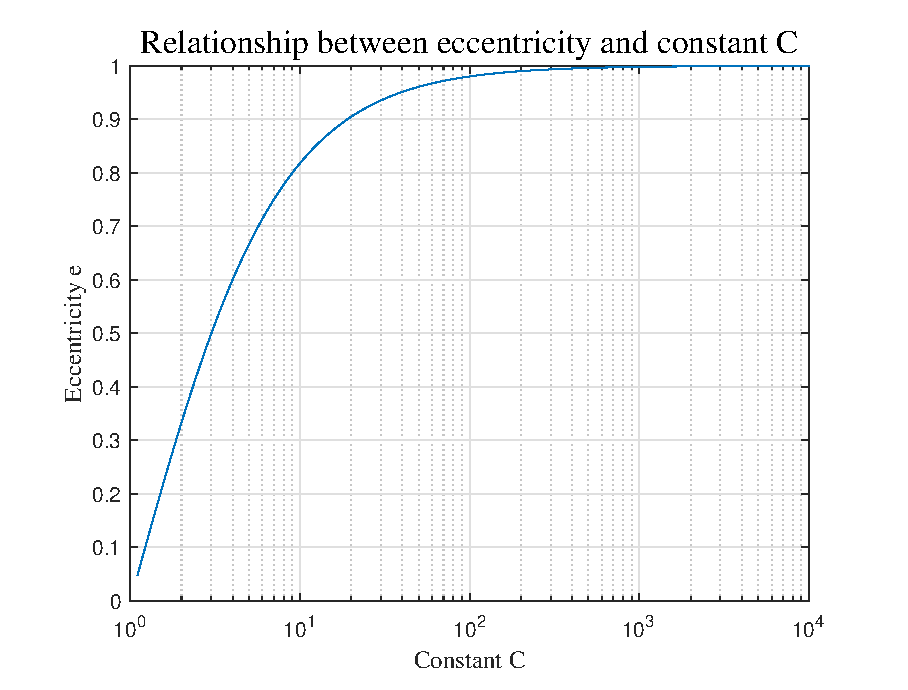
\includegraphics[width=0.9\linewidth]{Fig7.eps}
	\caption{The relationship between eccentricity $e$ and constant $C$.}	  
	\label{fig7} 
\end{figure}
Due to the line charge is positive, so the potential is not negative. So $C>1$ for $\ln{C}>0$. It can be seen from the monotonically increasing relationship of the logarithmic function that the larger the constant C, the larger the potential on the equipotential line. Therefore, we found that when the electric potential is small (where the area far away from the line charge), the eccentricity of the ellipse approaches 0, and the shape of the equipotential line tends to be circle ($e=0$). At the same time, the higher the potential, the closer the eccentricity is to 1 and the flatter the ellipse. And also, this result is consistent with Rowley's conclusion at polar coordinates.\cite{num3} 


\subsection{Error Analysis}
There is a certain error between the result obtained by the infinitesimal method and the true value. The error mainly depends on the number of segments divided by the line charge. Generally speaking, the more segments, the smaller the error.

First we introduce the concept of squared residuals $v^2$.Let $$v^2=(V-V_i)^2$$ $V$ is the real potential calculated by the integral method, $V_i$ is the electric potential approximated by the infinitesimal method.

In this way, we can infer the relative magnitude of the error between the results of the infinitesimal method and the true value through the value of the squares of the residuals.

However, due to the potentials at different points in the plane are different, in order to eliminate this effect, the normalized residual square is used to quantitatively describe the error.

We Define the normalized residual square is $v'$: $$v'=(\dfrac{V-V_i}{V})^2$$
The smaller $v'$ is, the closer the infinitesimal method result is to the true value.


\section{Results and Discussion}
\subsection{Calculus Method Result}
Using the results of calculus, in Matlab simulation, the potential, the potential and the electric field distribution of the finite line chargeas are shown in Fig. 2. 


\begin{figure}[H]   
	\centering	  
	\subfloat[]{       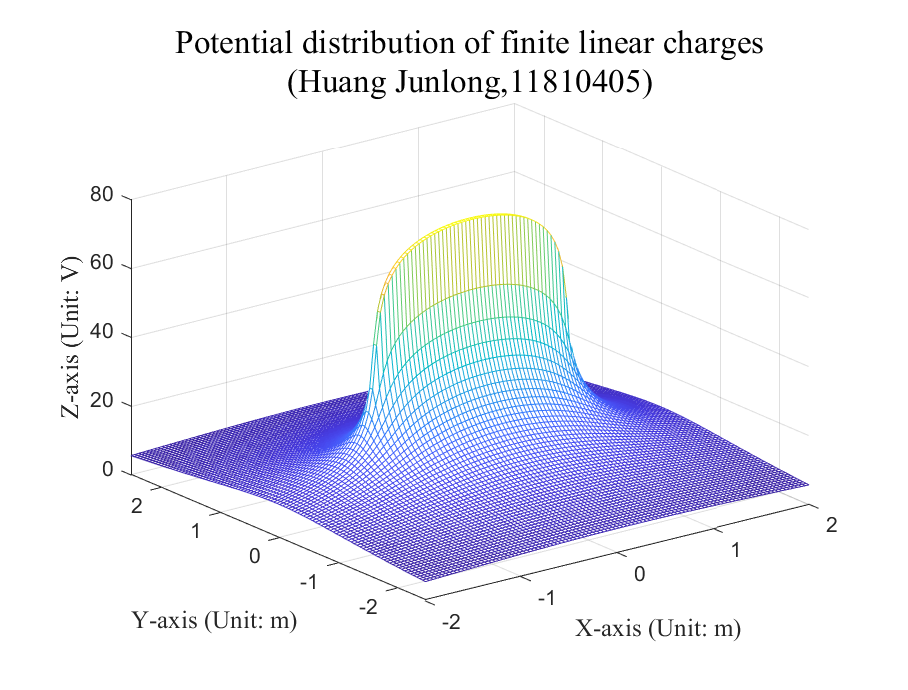
\includegraphics[width=0.45\linewidth]{Fig1-1.eps}}    \label{1a}\hfill	  
	\subfloat[]{        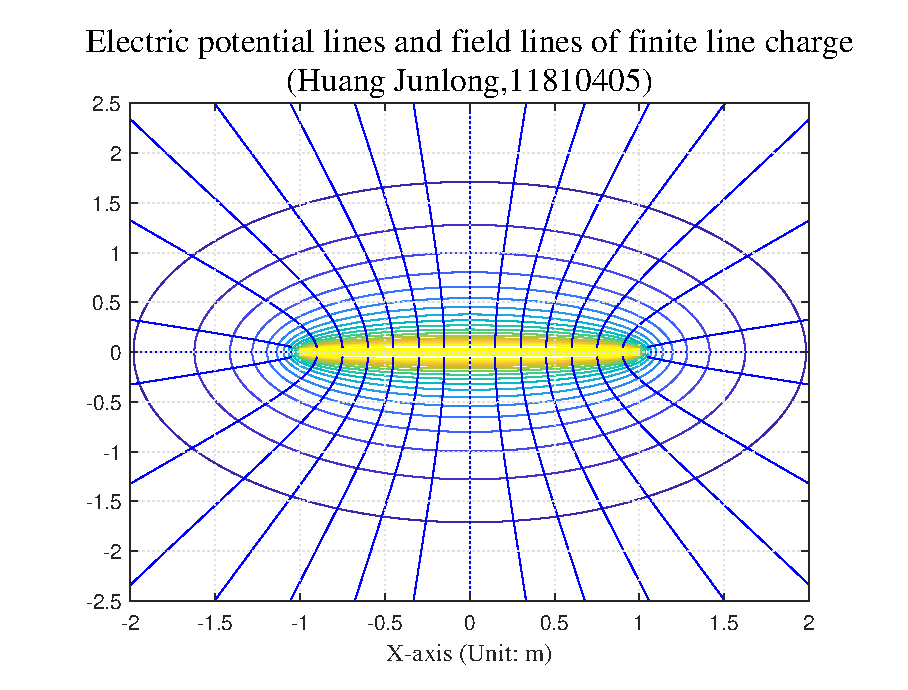
\includegraphics[width=0.45\linewidth]{Fig1-2.eps}}    
	\label{1b}
	\caption{Calculus Method Calculation results: (a) The potential of the finite line chargeas, (b) The electric field distribution of the finite line chargeas}	  
	\label{fig1} 
\end{figure}

From Fig. 2 (a), we can see the characteristics of finite line charge potential distribution: potential is a long bar, close to the position of the wire charge potential is high, far away from the line charge where the potential is low. At line charge intermediate accessory, the potential changes gently. At both ends of the line, the potential drops rapidly.
From Fig. 2 (b), it can be seen that the distribution of finite line charge electric field is indeed elliptical, as mentioned above. The area close to the line charge, the more flat the ellipse formed. The area away from the line charge, the more elliptical closer to the circle. At the same time, the electric field line is perpendicular to the isopotential face, like the electric field line of the point charge, dispersing in all directions.

\subsection{Infinitesimal Method Result}
Using the results of infinitesimal method, in Matlab simulation, the potential, the potential and the electric field distribution of the finite line chargeas are shown in Fig. 3 and Fig. 4 as follows.
\begin{figure}[H]   
	\centering	  
	\subfloat[Actuality]{       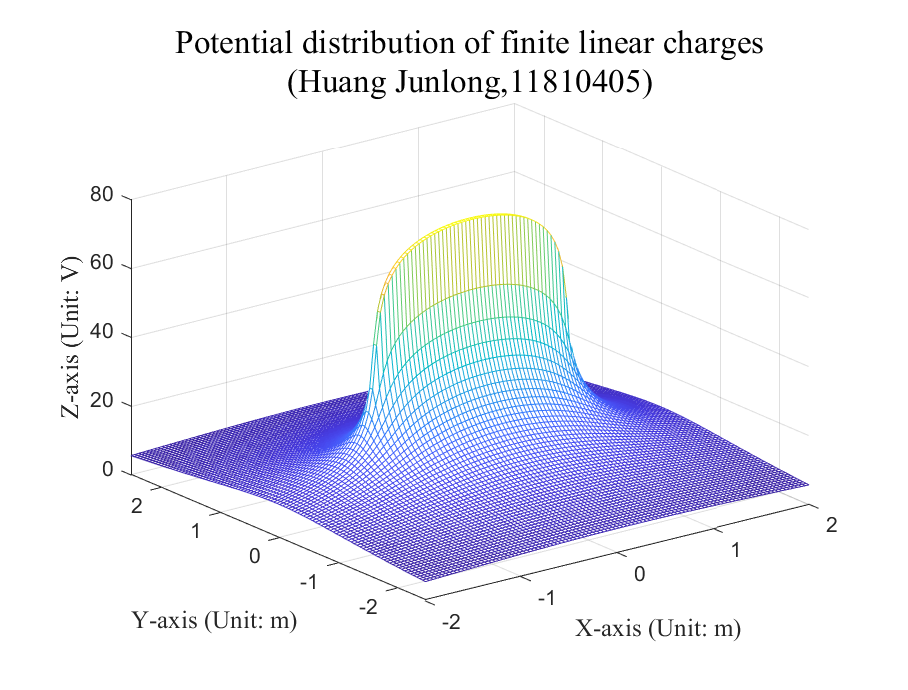
\includegraphics[width=0.45\linewidth]{Fig1-1.eps}}    \label{11}\hfill	  
	\subfloat[n=20]{        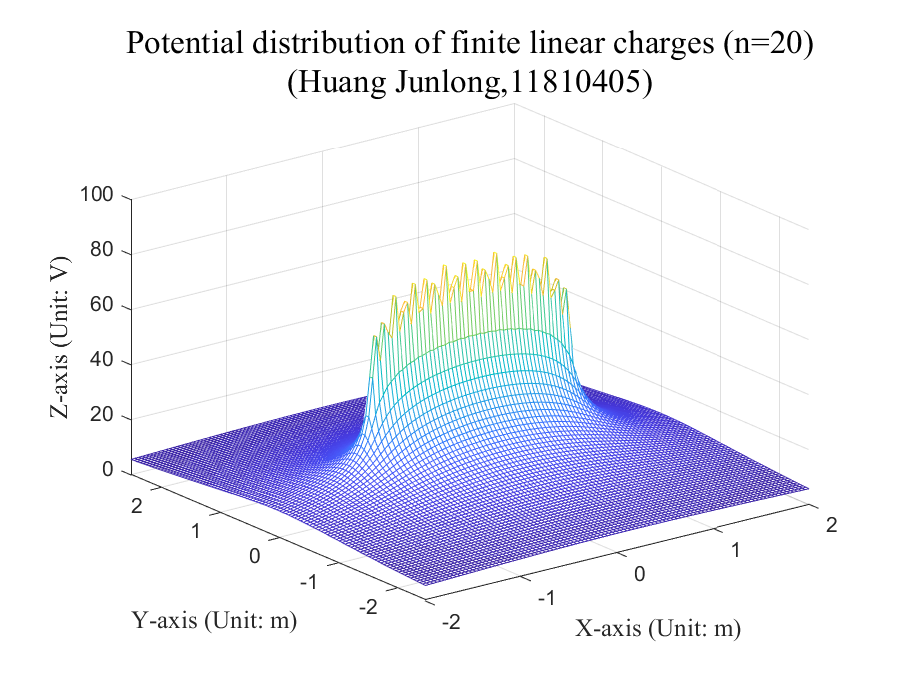
\includegraphics[width=0.45\linewidth]{Fig2-1.eps}}    
	\label{21}\\
	\subfloat[n=50]{       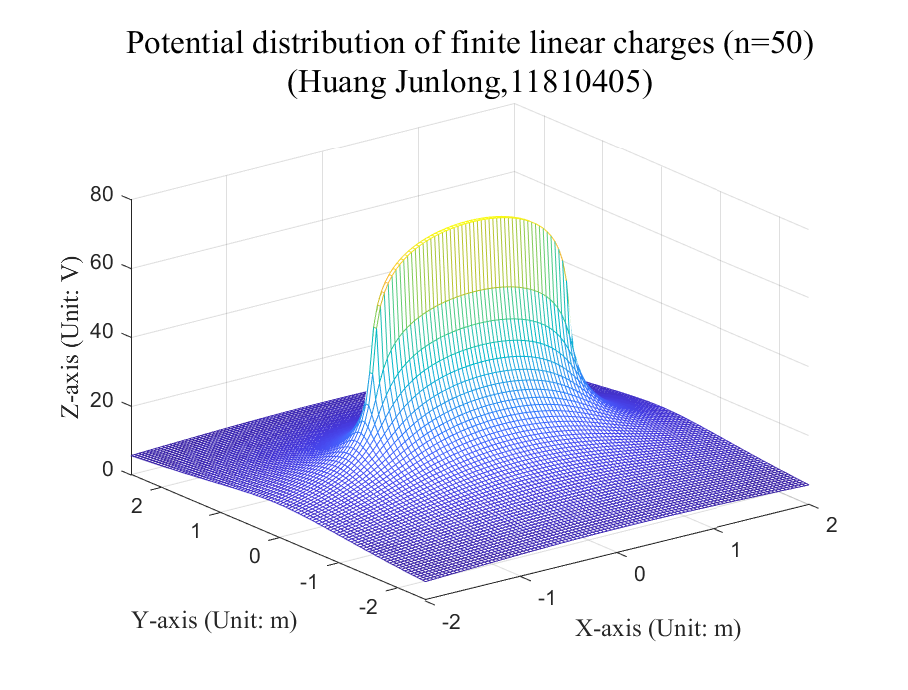
\includegraphics[width=0.45\linewidth]{Fig3-1.eps}}    \label{31}\hfill	  
	\subfloat[n=100]{        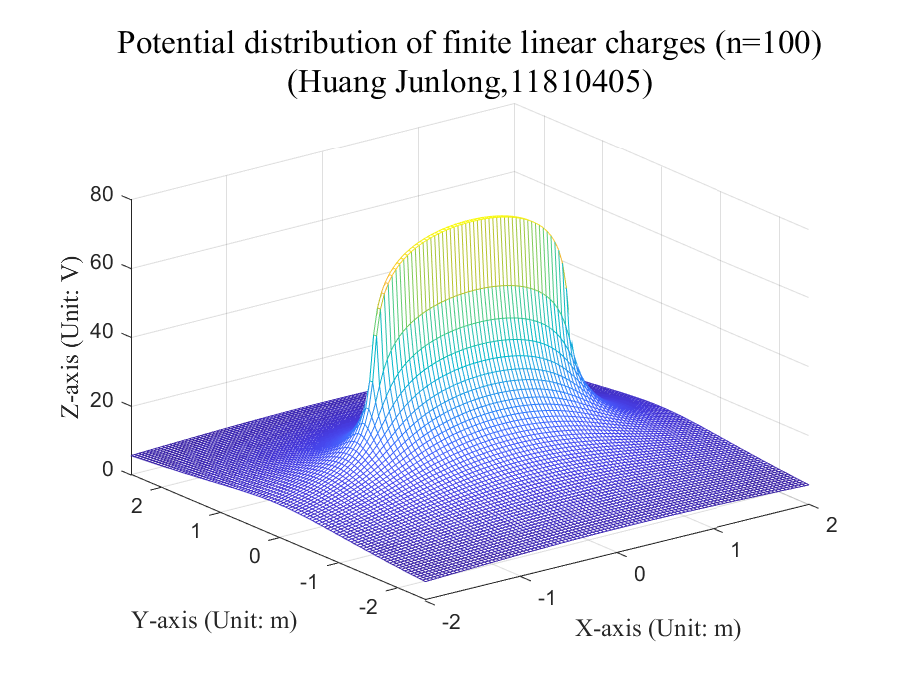
\includegraphics[width=0.45\linewidth]{Fig4-1.eps}}    
	\label{41}\\
	\caption{The potential distribution of the finite line chargeas (a) The actually result calculated by Calculus Method (b) The approximate result calculated by Infinitesimal Method when n=20 (c) n=50 (d) n=100
	}	  
	\label{fig3} 
\end{figure}
As can be seen from Fig. 3 (b), when the number of equal segments $n $is small, the potential distribution on the line charge is jagged. 
When $n$ is increased to 50 shown as Fig. 3 (c), the jagged becomes dense. When n is increased to 100 shown as Fig. 3 (d), the jagged edge become almost invisible. The infinitesimal method and the calculus method get almost the same graph. 
\begin{figure}[H]   
	\centering	  
	\subfloat[Actuality]{       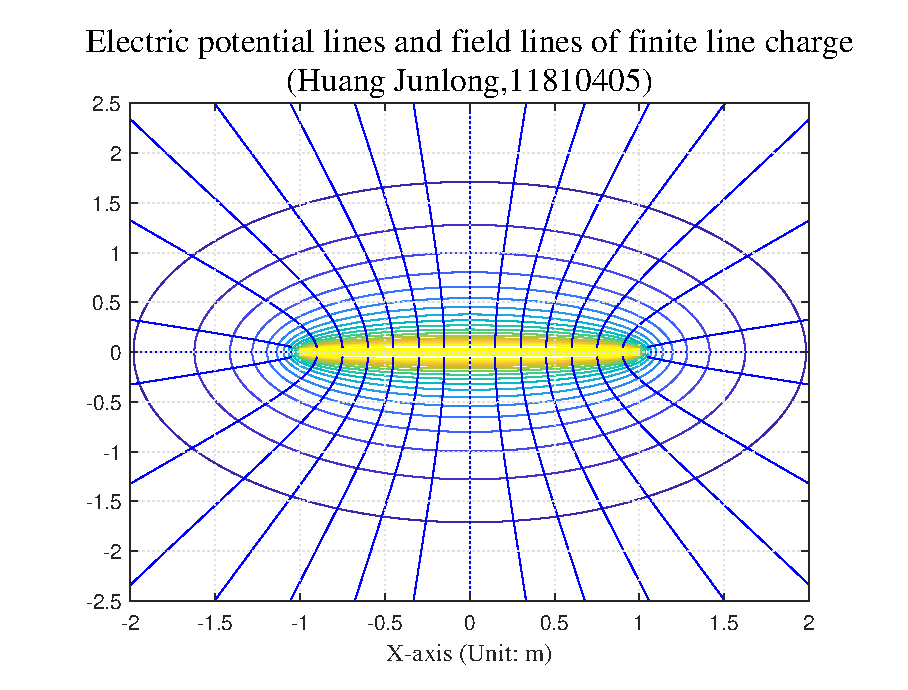
\includegraphics[width=0.45\linewidth]{Fig1-2.eps}}    \label{12}\hfill	  
	\subfloat[n=20]{        \includegraphics[width=0.45\linewidth]{Fig2-2.eps}}    
	\label{22}\\
	\subfloat[n=50]{       \includegraphics[width=0.45\linewidth]{Fig3-2.eps}}    \label{32}\hfill	  
	\subfloat[n=100]{        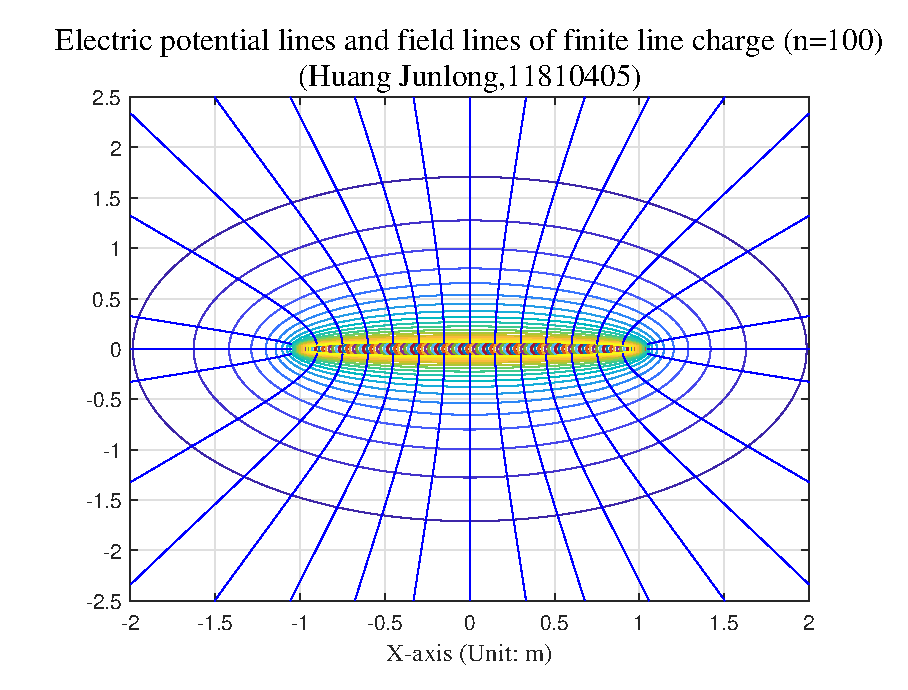
\includegraphics[width=0.45\linewidth]{Fig4-2.eps}}    
	\label{42}\\
	\caption{The potential and the electric field distribution of the finite line chargeas (a) The actually result calculated by Calculus Method (b) The approximate result calculated by Infinitesimal Method when n=20 (c) n=50 (d) n=100
	}	  
	\label{fig4} 
\end{figure}
Fig. 4 is the potential and the electric field distribution of the finite line chargeas in a two-dimensional plane. As n increases, the subdivision of point charge increases, and the potential surface of the ellipse becomes smoother. 

\subsection{Error Analysis Results}
Using the square residual method, the potential obtained by the infinitesimal was compared with the potential obtained by the calculus, the figures are as follows:
\begin{figure}[H]   
	\centering	  
	\subfloat[n=20]{       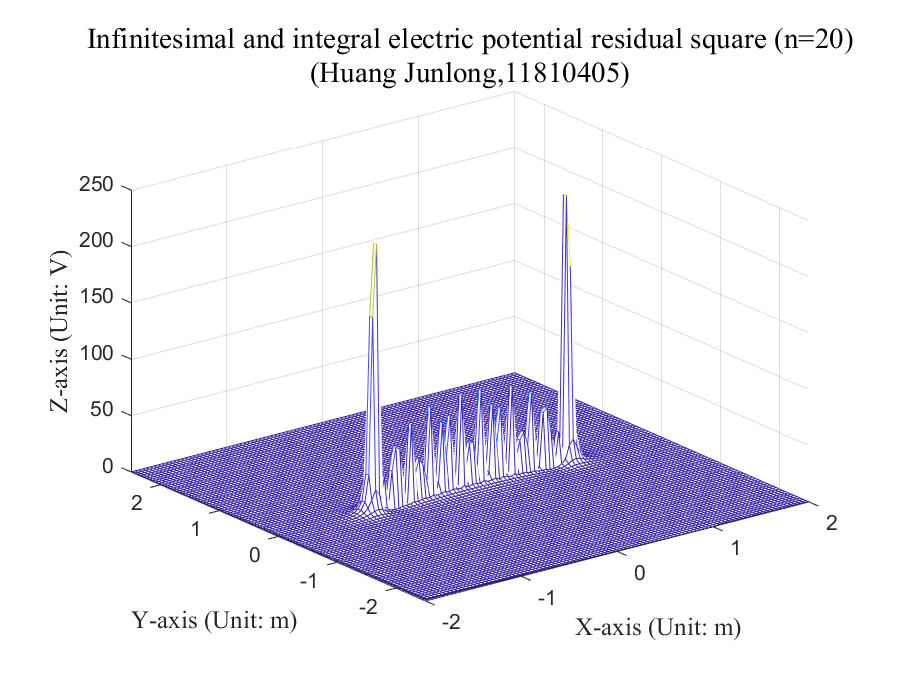
\includegraphics[width=0.45\linewidth]{Fig5-1.eps}}    \label{51}\hfill	  
	\subfloat[n=50]{        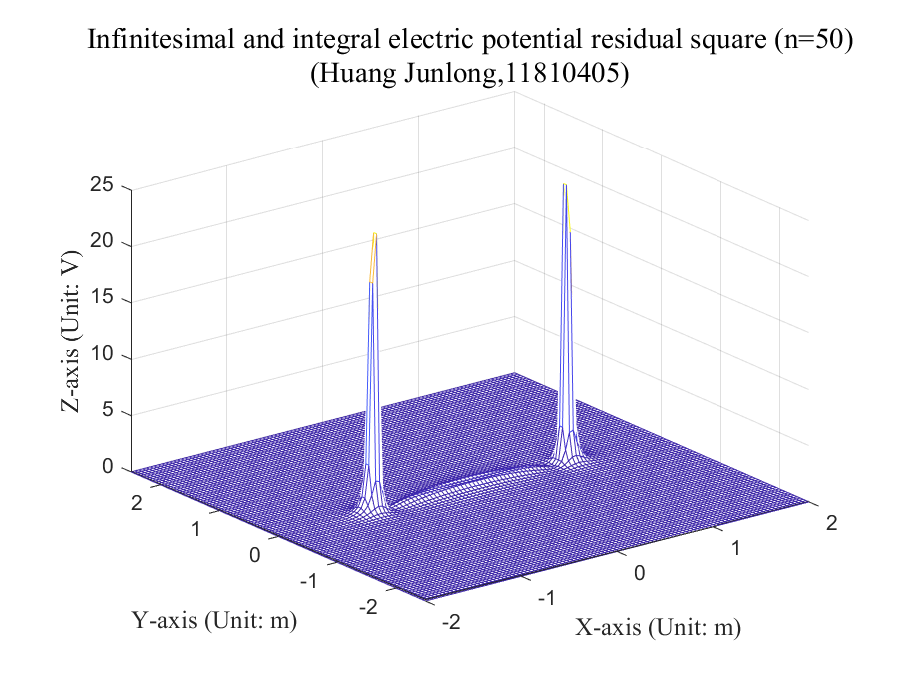
\includegraphics[width=0.45\linewidth]{Fig5-2.eps}}    
	\label{52}\hfill
	\subfloat[n=100]{       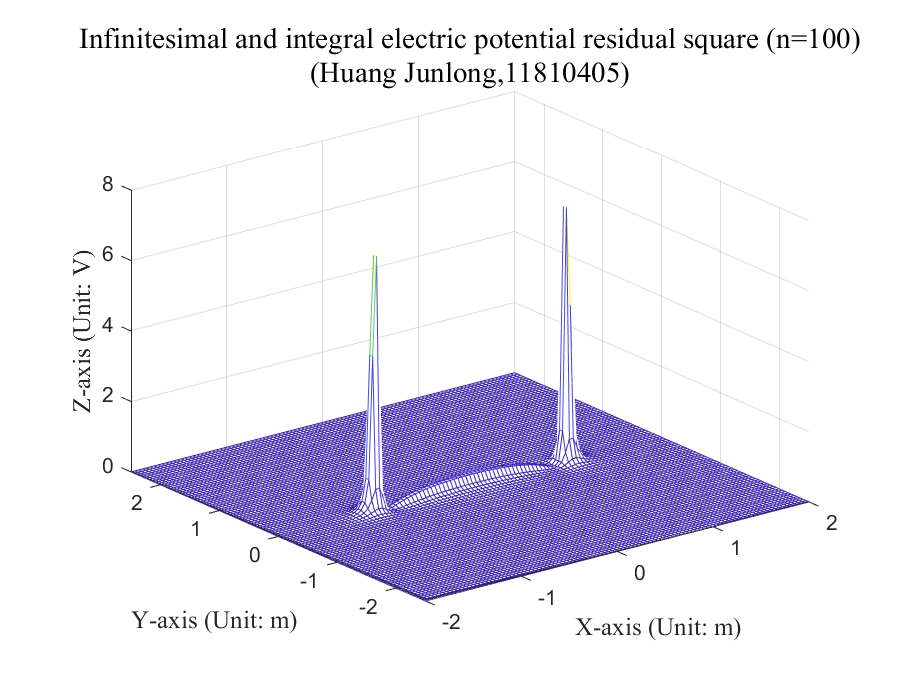
\includegraphics[width=0.45\linewidth]{Fig5-3.eps}}    \label{53}\hfill	  
	\caption{The square residual between infinitesimal and calculus (a) n=20 (b) n=50 (c) n=100
	}	  
	\label{fig5} 
\end{figure}
Since the actual potentials are different in different locations, and the z-axis ratioof of the three graphs is also different. In order to compare the results more directly and accurately, the residuals are normalized and squared, and the z-axis scale is set the same as the graph, the results are as follows.

\begin{figure}[H]   
	\centering	  
	\subfloat[n=20]{       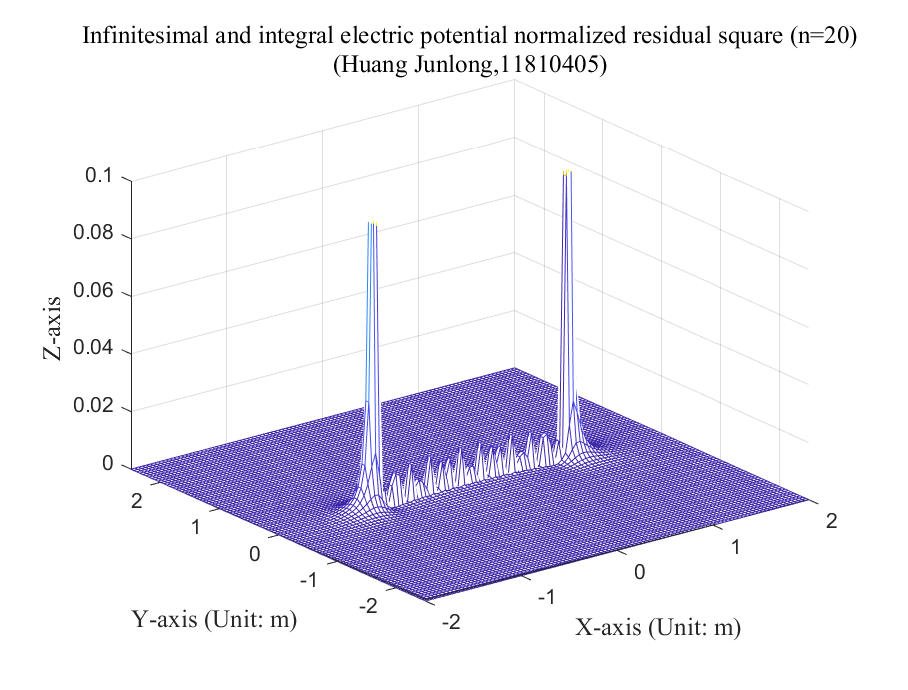
\includegraphics[width=0.45\linewidth]{Fig6-1.eps}}    \label{61}\hfill	  
	\subfloat[n=50]{        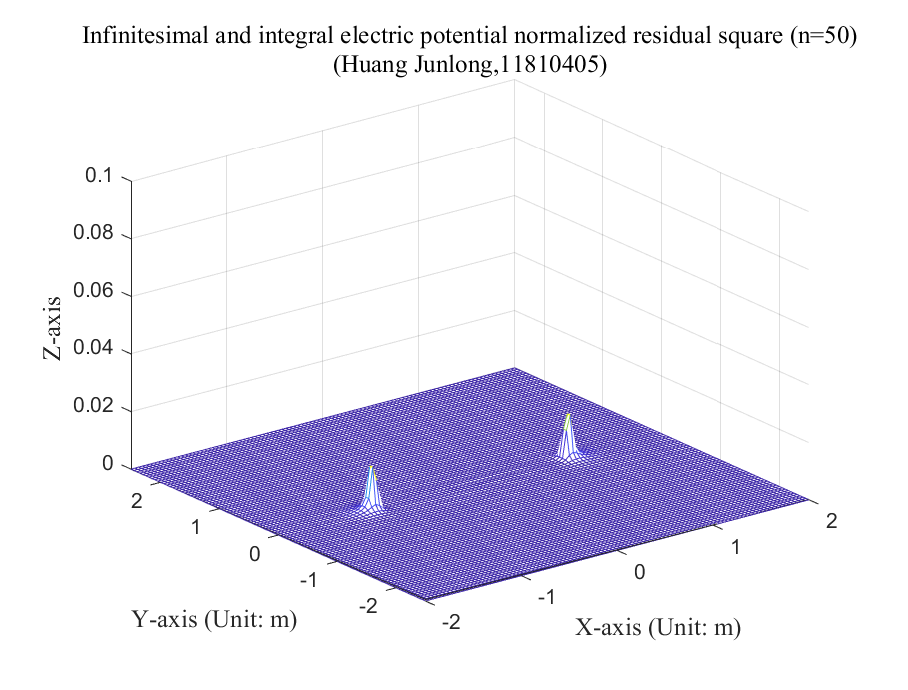
\includegraphics[width=0.45\linewidth]{Fig6-2.eps}}    
	\label{62}\hfill
	\subfloat[n=100]{       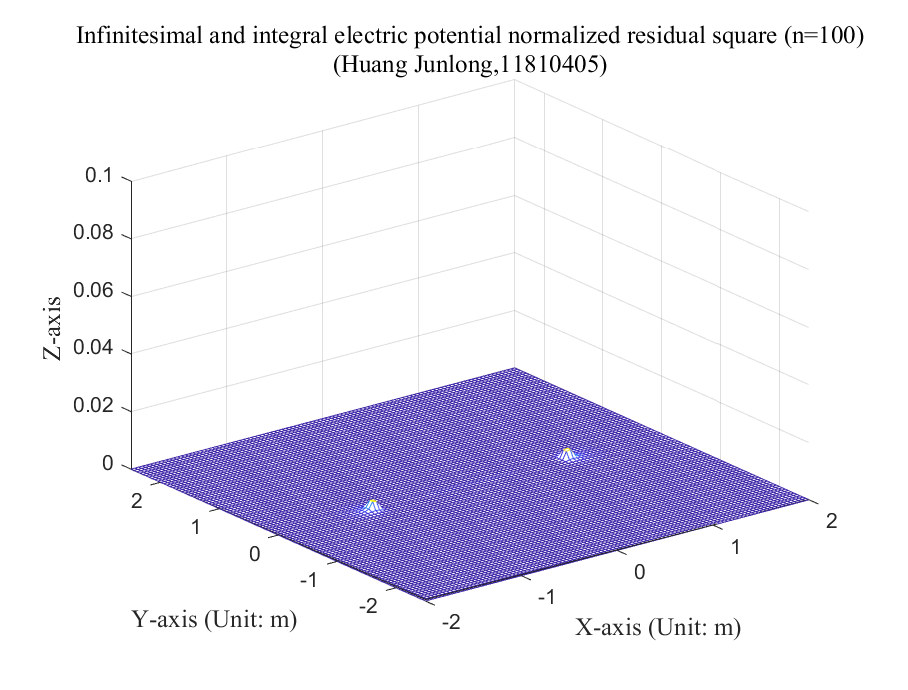
\includegraphics[width=0.45\linewidth]{Fig6-3.eps}}    \label{63}\hfill	  
	\caption{The square of normalized residual between infinitesimal and calculus (a) n=20 (b) n=50 (c) n=100
	}	  
	\label{fig5} 
\end{figure}

As can be seen from Fig. 5 (a), when $n=20$, the residual square is quite large, indicating that the results of the infinitesimal method calculation are very different from the actual result. The gap between infinitesimal method result and actual result is significantly smaller when n is 50 as shown in Fig. 5 (b). When $n=100$, only the two ends of the line charge have a little significantly difference as shown in Fig. 5 (c).

From Fig. 6, it can be seen more clearly that with the increase of n, the result of infinitesimal method and the actual result of the generalization residual smaller, the less error. That is, the more micro-meta-segments, the smaller the error with the real result. 

\section{Conclusion}
In this article, we use infinitesimal method and calculus method, respectively, to calculate the potential and electric field distribution of finite-length line charge, and to simulate and visualize in Matlab. Through calculation and simulation, we find that the isopotential plane of the finite length line charge is elliptically distributed, and the power line is perpendicular to the isopotential face from the line charge to the surrounding. 

At the same time, we introduce the concept of residual square, and quantitatively analyze the error between the result of infinitesimal method and the real value. It is verified that the more the number of microelements, the closer the result is to the true value. As can be seen from the Fig. 6, $n=50$ is an approximate processing value that reduces the calculation quantity to improve the computational efficiency without affecting too much the accuracy of the result.

Other calculation methods for finite-length wire charge electric fields and the best values for n will be expanded in subsequent work. 




\bibliographystyle{IEEEtran}
\bibliography{IEEEabrv,mylib}
%\begin{thebibliography}{2}

%\bibitem{IEEEhowto:kopka}
%H.~Kopka and P.~W. Daly, \emph{A Guide to \LaTeX}, 3rd~ed.\hskip 1em plus
%  0.5em minus 0.4em\relax Harlow, England: Addison-Wesley, 1999.

%\end{thebibliography}

% biography section
% 
% If you have an EPS/PDF photo (graphicx package needed) extra braces are
% needed around the contents of the optional argument to biography to prevent
% the LaTeX parser from getting confused when it sees the complicated
% \includegraphics command within an optional argument. (You could create
% your own custom macro containing the \includegraphics command to make things
% simpler here.)
%\begin{IEEEbiography}[{\includegraphics[width=1in,height=1.25in,clip,keepaspectratio]{mshell}}]{Michael Shell}
% or if you just want to reserve a space for a photo:



% You can push biographies down or up by placing
% a \vfill before or after them. The appropriate
% use of \vfill depends on what kind of text is
% on the last page and whether or not the columns
% are being equalized.

%\vfill

% Can be used to pull up biographies so that the bottom of the last one
% is flush with the other column.
%\enlargethispage{-5in}

% that's all folks
\newpage
\onecolumn 
\begin{appendices}
\section{}
\end{appendices}

\begin{lstlisting}
%% This is the code for Lab 2

%% Basic setup
clear all
clear;                    % Empty all variables in memory
clc;                      % Clear the contents of the command window
k=9e9;                    % Set the electrostatic force measure
rho=1e-9;                 % Set the charge density
xm=2;                     % Set the range in the x direction of the field
ym=2.5;                   % Set the range in the y direction of the field
x=linspace(-xm,xm,100);   % Divide the X-axis into 100 equal parts
y=linspace(-ym,ym,100);   % Divide the Y-axis into 100 equal parts
[X,Y]=meshgrid(x,y);      % Formed the coordinates of the points in the field

%% Calculus method
% Calculate the potential at each point in the field
V=k*rho.*log((1-X+sqrt((1-X).^2+Y.^2))./(-1-X+sqrt((-1-X).^2+Y.^2)));
% Plot the distribution of the potential
mesh(X,Y,V);
title({['Potential distribution of finite linear charges'],...
['(Huang Junlong,11810405)']},'FontName','Times New Roman','fontsize',16); 
xlabel('X-axis (Unit: m)','FontName','Times New Roman','fontsize',12);   
ylabel('Y-axis (Unit: m)','FontName','Times New Roman','fontsize',12);   
zlabel('Z-axis (Unit: V)','FontName','Times New Roman','fontsize',12);  
figure
Vmin=10;              % Set the minimum potential of the family of equipotential lines
Vmax=60;              % Set the maximum potential of the family of equipotential lines
Veq=linspace(Vmin,Vmax,18);        % Set the potential value of 18 equipotential lines
contour(X,Y,V,Veq);                % Draw 18 equipotential lines
grid on                            % Form a grid
hold on                            % Keep the graphics
line([-1,1],[0,0],'LineWidth',3,'color','y');  % Draw the line charge
% Calculate two components of the electric field intensity at each point in the field
[Ex,Ey]=gradient(-V); 
% Generate the X-axis coordinate of the starting point of the power line;
xs=linspace(-1.05,1.05,15);
% Generate the Y-axis coordinate of the starting point of the power line;
ys1=repmat(0.05,1,15);
ys2=repmat(-0.05,1,15);
% Generating power lines;
streamline(X,Y,Ex,Ey,xs,ys1);
streamline(X,Y,Ex,Ey,xs,ys2);
streamline(X,Y,Ex,Ey,-1.05,0);
streamline(X,Y,Ex,Ey,1.05,0);
title({['Electric potential lines and field lines of finite line charge'],...
['(Huang Junlong,11810405)']} ,'FontName','Times New Roman', 'fontsize', 16);      
xlabel('X-axis (Unit: m)','FontName','Times New Roman','fontsize',12);  

%% Infinitesimal method
qi=zeros(1,3);                  % Set micro-point charges
ni=[20,50,100];                 % Set the number of equal parts of the line charge        
Error=zeros(100,100,3);         % Use residuals as errors
ErrorNor=zeros(100,100,3);      % Use normalized residuals as errors
xqi=zeros(1,100,3);             % Initialization the micro-point charges x coordinate
% Set thr micro-point charges x coordinate
xqi(:,:,1)=[linspace(-1,1,20),zeros(1,80)];  
xqi(:,:,2)=[linspace(-1,1,50),zeros(1,50)];
xqi(:,:,3)=[linspace(-1,1,100)];
V1=zeros(100,100);              % Initialization the electric potential
for m=1:3                       % Set for loop for 3 cases
figure
qi(m)=rho*2/ni(m);          % Calculate the amount of point charge
for i=1:ni(m)
% Calculate the potential generated by the point charge at each point
Vi=k*qi(m)./sqrt((X-xqi(1,i,m)).^2+Y.^2);  
% Sum up to get the potential generated by the entire line charge
V1=V1+Vi;
end
mesh(X,Y,V1);               % Plot the distribution of the potential
title({['Potential distribution of finite linear charges (n=' num2str(ni(m)) ')'],...
['(Huang Junlong,11810405)']},'FontName','Times New Roman','fontsize',16); 
xlabel('X-axis (Unit: m)','FontName','Times New Roman','fontsize',12);   
ylabel('Y-axis (Unit: m)','FontName','Times New Roman','fontsize',12);   
zlabel('Z-axis (Unit: V)','FontName','Times New Roman','fontsize',12);  
figure
for n=1:ni(m)              
plot(xqi(1,n,m),0,'o', 'MarkerSize',5)  % Draw n point charges
hold on
end
Vmin=10;             % Set the minimum potential of the family of equipotential lines
Vmax=60;             % Set the maximum potential of the family of equipotential lines
Veq=linspace(Vmin,Vmax,18);       % Set the potential value of 18 equipotential lines
contour(X,Y,V1,Veq);              % Draw 18 equipotential lines
hold on
grid on
[Ex,Ey]=gradient(-V); 
xs=linspace(-1.05,1.05,15);
ys1=repmat(0.05,1,15);
ys2=repmat(-0.05,1,15);
% Generating power lines;
streamline(X,Y,Ex,Ey,xs,ys1);
streamline(X,Y,Ex,Ey,xs,ys2);
streamline(X,Y,Ex,Ey,-1.05,0);
streamline(X,Y,Ex,Ey,1.05,0);
title({['Electric potential lines and field lines of finite line charge (n=' num2str(ni(m)) ')'],...
['(Huang Junlong,11810405)']} ,'FontName','Times New Roman', 'fontsize', 15);      
xlabel('X-axis (Unit: m)','FontName','Times New Roman','fontsize',12);
% Calculate the sum of squared residuals. 
% between the infinitesimal and the integrated potential
Error(:,:,m)=(V1-V).^2;
% Calculate the sum of squared normalized residuals. 
% between the infinitesimal and the integrated potential
ErrorNor(:,:,m)=((V1-V)./V).^2;
% Clear and reset the voltage at each point of the planar field
clear Vi;
V1=zeros(100,100);
end

%% Error Analysis
% Infinitesimal and integral electric potential residual square
for k=1:3
figure
mesh(X,Y,Error(:,:,k));               
% axis([-2 2,-2.5,2.5,0 200])
title({['Infinitesimal and integral electric potential residual square (n=' num2str(ni(k)) ')'],...
['(Huang Junlong,11810405)']},'FontName','Times New Roman','fontsize',14); 
xlabel('X-axis (Unit: m)','FontName','Times New Roman','fontsize',12);   
ylabel('Y-axis (Unit: m)','FontName','Times New Roman','fontsize',12);   
zlabel('Z-axis (Unit: V)','FontName','Times New Roman','fontsize',12);
end
% Infinitesimal and integral electric potential normalized residual square
for k=1:3
figure
mesh(X,Y,ErrorNor(:,:,k));             
axis([-2 2,-2.5,2.5,0 0.1])
title({['Infinitesimal and integral electric potential normalized residual square (n=' ...
num2str(ni(k)) ')'],['(Huang Junlong,11810405)']},'FontName','Times New Roman','fontsize',12); 
xlabel('X-axis (Unit: m)','FontName','Times New Roman','fontsize',12);   
ylabel('Y-axis (Unit: m)','FontName','Times New Roman','fontsize',12);   
zlabel('Z-axis ','FontName','Times New Roman','fontsize',12);
end

%% The calculation of elliptical eccentricity
clc,clear
xn=linspace(1,1e4,1e5);
y=sqrt(1-(4.*xn.*(xn-1).^2)./((xn.^2-1).^2));
plot(xn,y)
semilogx(xn,y)
grid on
xlabel('Constant C','FontName','Times New Roman','fontsize',12)
ylabel('Eccentricity e','FontName','Times New Roman','fontsize',12)
title('Relationship between eccentricity and constant C','FontName','Times New Roman','fontsize',16)
\end{lstlisting}


\end{document}

